%%
% このファイルは、筑波大学情報学群情報科学類の
% 卒業研究論文本体のサンプルです。
% このファイルを書き換えて、この例と同じような書式の論文本体を
% LaTeXを使って作成することができます。
% 
% PC環境や、LaTeX環境の設定によっては漢字コードや改行コードを
% 変更する必要があります。
%%
\documentclass[a4paper,11pt,dvipdfmx]{jreport}

%%【PostScript, JPEG, PNG等の画像の貼り込み】
%% 利用するパッケージを選んでコメントアウトしてください。
\usepackage{graphicx} % for \includegraphics[width=3cm]{sample.eps}
%\usepackage{epsfig} % for \psfig{file=sample.eps,width=3cm}
%\usepackage{epsf} % for \epsfile{file=sample.eps,scale=0.6}
%\usepackage{epsbox} % for \epsfile{file=sample.eps,scale=0.6}

%% dvipdfm を使う場合(dvi->pdfを直接生成する場合)
%\usepackage[dvipdfm]{color,graphicx}
%% dvipdfm を使ってPDFの「しおり」を付ける場合
%\usepackage[dvipdfm,bookmarks=true,bookmarksnumbered=true,bookmarkstype=toc]{hyperref}
%% 参考:dvipdfm 日本語版
%% http://hamilcar.phys.kyushu-u.ac.jp/~hirata/dvipdfm/

\usepackage[bookmarksnumbered=true]{hyperref}
\usepackage{pxjahyper}

\usepackage{times} % use Times Font instead of Computer Modern

\setcounter{tocdepth}{3}
\setcounter{page}{-1}

\setlength{\oddsidemargin}{0.1in}
\setlength{\evensidemargin}{0.1in} 
\setlength{\topmargin}{0in}
\setlength{\textwidth}{6in} 
%\setlength{\textheight}{10.1in}
\setlength{\parskip}{0em}
\setlength{\topsep}{0em}

%\newcommand{\zu}[1]{{\gt \bf 図\ref{#1}}}

%% タイトル生成用パッケージ(重要)
\usepackage{coins-jp}
\usepackage{jumoline}

%% タイトル
%% 【注意】タイトルの最後に\\ を入れるとエラーになります
\title{\Underline{Containerless:オブジェクトシステムの新しいとらえ方}}
%% 著者
\author{林 拓人}
%% 指導教員
\advisor{前田敦司}

%% 専攻名 と 年月 (提出年月)
%% 年月は必要に応じて書き替えてください。
\heiseiyear{26}  % 平成の年度
\majorfield{ソフトウェアサイエンス主専攻}
%\majorfield{情報システム主専攻}
%\majorfield{知能情報メディア主専攻}


\begin{document}
\maketitle
\thispagestyle{empty}
\newpage

\thispagestyle{empty}
\vspace*{20pt plus 1fil}
\parindent=1zw
\noindent
%%
%% 論文の概要(Abstract)
%%
\begin{center}
{\Large \bf 要  旨}
\vspace{2cm}
\end{center}
[400字程度]

%%%%%
\par
\vspace{0pt plus 1fil}
\newpage

\pagenumbering{roman} % I, II, III, IV 
\tableofcontents
\listoffigures
%\listoftables

\pagebreak \setcounter{page}{1}
\pagenumbering{arabic} % 1,2,3


\chapter{序論}

オブジェクトシステムとは,\textbf{オブジェクト指向プログラミング}\cite{Stroustrup:1988:OP:624569.624721}
を支援するプログラミング言語の機構である.
本研究は従来のオブジェクトシステムを分析し考案した,新しいモデルに基づくオブジェクトシステムを提案する.
従来とは異なるモデルを示すことで,オブジェクトシステムにまつわる既存の概念に対し新たな見方を提供することが
目的である.

[ここで論文の構成について述べる]


\chapter{従来のオブジェクトシステム}

本章ではクラスを用いてメソッドディスパッチをする従来のオブジェクトシステムをモデル化する.

\section{クラスにメソッドを定義するモデル}

C++,Java,Smalltalk,Ruby

\section{総称関数にメソッドを定義するモデル}

Common Lisp,Dylan

\begin{figure}[htbp]
\begin{center}
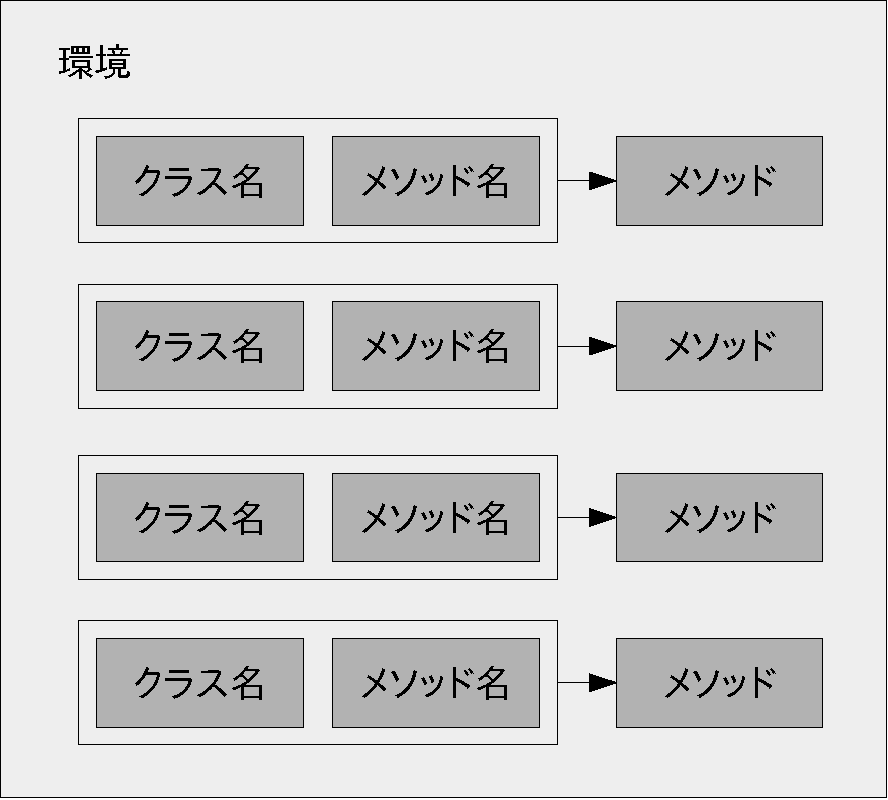
\includegraphics[width=3cm]{fig/environment-crop.pdf}
%\psfig{file=sample.eps,scale=0.6}
%\epsfile{file=sample.eps,scale=0.6}
\end{center}
\caption{図の例}
\label{figure:sample}
\end{figure}

\chapter{落ち穂拾い}

\begin{enumerate}
\item プロトタイプベースの方が動的
\item 静的型検査は型クラスみたいにしてできそう
\item Clojureのマルチメソッドはオブジェクトシステムからポリモーフィズムだけを抽出したもの
\end{enumerate}

\chapter{結論}

知見を得た

\chapter*{謝辞}
\addcontentsline{toc}{chapter}{\numberline{}謝辞}

\newpage

\addcontentsline{toc}{chapter}{\numberline{}参考文献}
\renewcommand{\bibname}{参考文献}

%% 参考文献に jbibtex を使う場合
\bibliographystyle{junsrt}
\bibliography{thesis}
%% [compile] jbibtex sample; platex sample; platex sample;

%% 参考文献を直接ファイルに含めて書く場合
%\begin{thebibliography}{1}
%\bibitem{RakRak}
%野寺隆志.
%\newblock 楽々 \LaTeX.
%\newblock 共立出版, 1990.
%
%\bibitem{JiyuuJizai}
%磯崎秀樹.
%\newblock \LaTeX 自由自在.
%\newblock サイエンス社, July 1992.
%
%\bibitem{bryant-ieeetc86}
%Randal~E. Bryant.
%\newblock Graph-based algorithms for {B}oolean function manipulation.
%\newblock {\em IEEE Transactions on Computers}, Vol. C-35, No.~8, pp. 677--691,
%  August 1986.
%\end{thebibliography}

\end{document}
